\documentclass[11pt]{article}
\usepackage[margin=0.7in]{geometry}
\usepackage{booktabs,graphicx,hyperref}
\hypersetup{colorlinks=true,urlcolor=blue}
\emergencystretch=3em
\title{Impala Step 9: GPU execution and coordination}
\author{Measurement of the step-8 experimental path}
\date{September 30, 2026}
\begin{document}\maketitle
\section*{Experiment and accuracy}
This is instrumentation only. Sampler, kernels, transfers and synchronous
scheduling policy remain unchanged. Four independent standard chains use seeds
42/123/456/789, 3,000 states and 50 temperatures. An exploratory larger-call
sweep uses eight independent chains, 1,000 states and the same 50 temperatures.
The additional seeds are 1011/1213/1415/1617. All saved outputs,
including full-temperature arrays, match exactly across instrumentation modes.
The standard plain run also matches the recorded step-8 GPU candidate exactly.
The original prediction fixture is checked at every launch. 19 passed in 5.64s

There is no new long posterior-quality study: this experiment measures unchanged
computation. Short eight-chain runs do not establish convergence or an
ESS/s comparison with the standard workload. No production default changes.
An initial 200-temperature attempt failed before sampling: the existing ladder
yields a negative Gamma shape during warm-up. Its logs are preserved; larger
batches instead use more independent chains without changing the sampler.
\section*{Instrumentation overhead}
No cProfile is used. Coordination timers separate polling, receive/decode,
assembly/split, model evaluation and sends, and record worker request timestamps.
Detailed GPU timing additionally uses CUDA events and stage synchronization.
Three standard rounds rotate mode order, with no overlapping runs. Seconds below
are elapsed group sampling time; startup/JIT and saving are excluded, while cache
misses, CPU work, transfers and coordination remain included.
\begin{center}\begin{tabular}{lrrrr}\toprule
Mode & Round 1 & Round 2 & Round 3 & Median\\\midrule
plain & 10.726 & 10.811 & 10.841 & 10.811\\
coordination & 10.801 & 10.740 & 10.847 & 10.801\\
stages & 11.052 & 10.964 & 11.158 & 11.052\\
\bottomrule\end{tabular}\end{center}
Coordination median/plain ratio: 0.999; detailed-stage median/plain ratio:
1.022. These ratios include timing variation, not just instrumentation cost.
Larger-call times (one run each): plain 4.923 s, coordination 5.025 s,
detailed stages 5.047 s. They are exploratory, not repeated speed estimates.
\section*{Nonoverlapping coordinator wall-time breakdown}
The figure uses standard detailed-stage round 2 and the larger detailed-stage run.
Each bar totals elapsed group time. Device event durations are nested within model
wall time and subtracted from other model time; they are never counted twice.
\begin{center}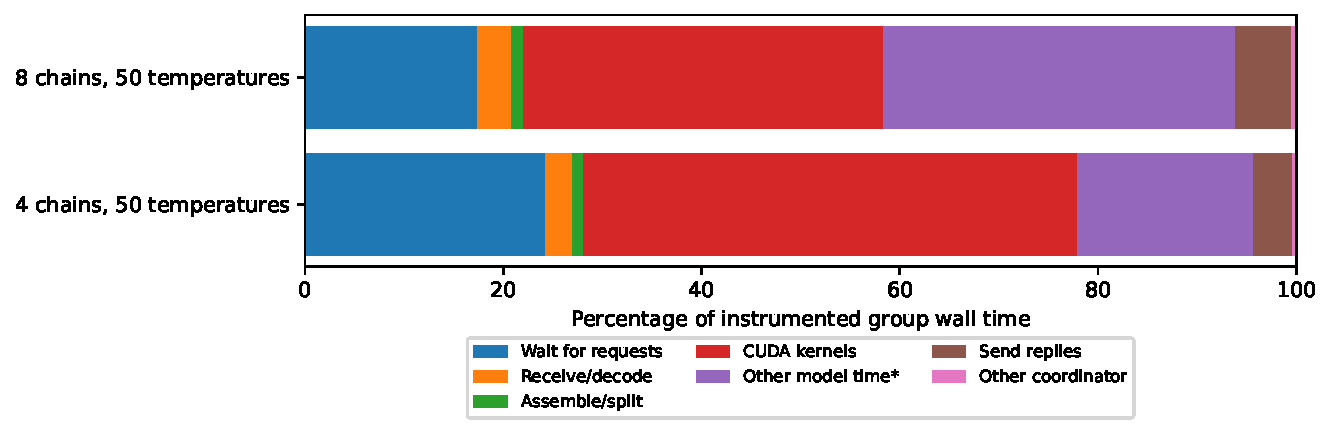
\includegraphics[width=0.94\linewidth]{step9-breakdown.pdf}\end{center}
\noindent *Other model time includes host validation, cache preparation, transfers,
allocation, launches and synchronization outside measured history/interpolation
kernel intervals. It is not all avoidable overhead. Kernel time/wall time is not
hardware occupancy, and these fractions describe instrumented runs.
\begin{center}\begin{tabular}{lrr}\toprule
Component & 4 chains (s) & 8 chains (s)\\\midrule
Wait for requests & 2.663 & 0.877\\
Receive/decode & 0.293 & 0.173\\
Assemble/split & 0.127 & 0.065\\
CUDA kernels & 5.460 & 1.829\\
Other model time* & 1.951 & 1.792\\
Send replies & 0.430 & 0.286\\
Other coordinator & 0.040 & 0.025\\
\bottomrule\end{tabular}\end{center}
\section*{Interpretation}
In the illustrated standard run, CUDA history/interpolation kernels occupy
49.8 percent of elapsed time; request polling occupies 24.3 percent,
and receiving/decoding plus sending replies occupy 6.6 percent. In the
larger-call run, kernel time accounts for 36.2 percent. The detailed
JSON separates geometry preparation, parameter expansion/upload and output download.
Geometry preparation/upload takes 4.5 percent of standard elapsed time
and 23.6 percent in the larger-call run. The latter includes
1.028 s of first-observed cache misses and 0.141 s of repeated
misses. Its shorter duration makes first-use costs proportionally larger;
this is not proof of a sustained 24-percent geometry cost in long runs.
These measurements support examining the history kernel and model-side setup
before rewriting communication. Poll waiting cannot simply be removed: workers
must compute their next sampler transition after each result. Asynchronous
scheduling might overlap some work, but smaller GPU batches and new coordination
costs could offset that gain; no asynchronous speedup has been demonstrated.
\section*{Worker skew and request waiting}
In coordination-only standard round 2, request-start spread across workers has
median 0.132 ms and p95 0.220 ms. Latest-request-to-model-start median is
0.164 ms (p95 0.294 ms). Combined parameter batch size averages 159.1
(p95 200.0). Larger coordination-only requests average 332.7 parameters.

A timestamp precedes worker serialization. Request-to-model latency therefore
includes serialization, pipes, scheduling, waiting for peers and assembly.
Polling waits include necessary sampler work. Worker request waits overlap each
other and the GPU; do not add them to parent wall time. Request spread is not
an additive cost or an asynchronous speedup estimate. Parent CPU time and each
worker's inside/outside-request wall and CPU time are retained in the JSON.
\section*{Reproduction and tracking}
\begingroup\small\raggedright
Measured commit: \texttt{694fd8d}. Branch: \texttt{perf/gpu-coordination-profile};
checkpoint: \texttt{perf-step9-20260930}. Authored by Ayan Biswas
\texttt{<ayanju04@gmail.com>}; no push. See \path{docs/performance/STEP9.md} for
interpretation and commands. \path{benchmarks/gpu_coordination_suite.py} runs
controls; \path{benchmarks/gpu_coordination_report.py} rebuilds this report.
JSON, plot PDF, LaTeX, tests and SHA-256 inventory are versioned under
\path{docs/performance/results/step9*}; raw traces and samples reside in workspace
\path{benchmark/changes/step9/}. Hardware: Core Ultra 9 285HX, RTX PRO 5000
Blackwell laptop GPU. Mac testing, hierarchical mixing and asynchronous scheduling
remain separate. See the accompanying Markdown findings for the next experiment.
\par\endgroup
\end{document}
